\documentclass[11pt,a4paper]{article}
\usepackage[utf8]{inputenc}
\usepackage[T1]{fontenc}
\usepackage[spanish,es-nodecimaldot]{babel}
\usepackage{helvet}
\renewcommand{\familydefault}{\sfdefault}
\usepackage[margin=2.5cm]{geometry}
\usepackage{graphicx,booktabs,xcolor,float,amsmath,enumitem,array,caption,fancyhdr}
\usepackage[hidelinks]{hyperref}
\definecolor{gris}{RGB}{90,90,90}
\definecolor{titulo}{RGB}{38,50,62}
\newcommand{\pendiente}[1]{\textcolor{red}{[PENDIENTE: #1]}}
\captionsetup{font=small,labelfont=bf}
\setlength{\parskip}{4pt}
\setlist{itemsep=2pt,topsep=2pt}
\pagestyle{fancy}
\fancyhf{}
\renewcommand{\headrulewidth}{0pt}
\fancyfoot[L]{\footnotesize\color{gris} Segmentación de nube de puntos de fábrica · Grupo 4 · Machine Learning, UTEC}
\fancyfoot[R]{\footnotesize\color{gris} Pág. \thepage}

\begin{document}
\begin{titlepage}
\thispagestyle{empty}
\centering
\vspace*{0.5cm}
{\large\bfseries UNIVERSIDAD DE INGENIERÍA Y TECNOLOGÍA\par}
\vspace{1.2cm}

\includegraphics[width=4.2cm]{logo_utec.png}\par
\vspace{1.6cm}
{\fontsize{24}{28}\selectfont\bfseries\color{titulo} Segmentación de una nube de puntos de fábrica con clustering en múltiples etapas\par}
\vspace{0.5cm}
{\normalsize\color{gris} Actividad 3\par}
\vspace{1.4cm}
{\small\bfseries\color{gris} GRUPO\par}\vspace{0.3cm}
{\small Grupo 4\par}
\vspace{0.8cm}
{\small\bfseries\color{gris} INTEGRANTES\par}\vspace{0.4cm}
{\small
Zheng Chan, Enrique \hspace{4pt}|\hspace{4pt} \pendiente{código}\par\vspace{2pt}
Limaco Porras, Requelmy \hspace{4pt}|\hspace{4pt} \pendiente{código}\par\vspace{2pt}
León Pantaleón, Jobeth Alexander \hspace{4pt}|\hspace{4pt} 202510035\par\vspace{2pt}
Huamán Huamaní, Josué Yeremi \hspace{4pt}|\hspace{4pt} \pendiente{código}\par}
\vspace{0.9cm}
{\small\bfseries\color{gris} CURSO\par}\vspace{0.3cm}
{\small\bfseries\color{gris} Machine Learning\par}
\vspace{1.2cm}
{\small Lima, Perú \hspace{4pt}|\hspace{4pt} Noviembre de 2026\par}
\end{titlepage}

\section*{Resumen del trabajo y entregables}
\begin{tabular}{@{}p{6.2cm}p{8.8cm}@{}}
\toprule
\textbf{Integrante} & \textbf{Rol} \\
\midrule
Zheng Chan, Enrique & Rol 3 · Etapa 2: objetos \\
Limaco Porras, Requelmy & Rol 4 · Integración, evaluación y reporte \\
León Pantaleón, Jobeth Alexander & Rol 1 · Datos y preprocesamiento \\
Huamán Huamaní, Josué Yeremi & Rol 2 · Etapa 1: estructura global \\
\bottomrule
\end{tabular}

\medskip
\noindent\textbf{Repositorio (código fuente):} \url{https://github.com/AIexander-lx/segmentacion-nube-puntos} (rama \texttt{main}).

\noindent\textbf{Entregables:} este reporte en PDF, el código en el repositorio y la nube de puntos coloreada por clase (\texttt{fabrica\_segmentada.ply}).

\tableofcontents
\newpage

\section{Introducción y objetivo}
El objetivo es segmentar los objetos de una nube de puntos 3D de una fábrica (columnas, vigas, tuberías, piso, techo y paredes, entre otros) y exportar la nube con un color por punto según la clase identificada. La consigna recomienda combinar algoritmos de clustering en varias etapas, aprovechando los atributos disponibles: posición, color RGB y normal.

La solución sigue un esquema en cuatro bloques: (i) preprocesamiento por voxel y filtrado de ruido; (ii) etapa 1, detección de superficies planas grandes con RANSAC; (iii) etapa 2, agrupamiento espacial de los puntos restantes, descriptores de forma por PCA y clasificación por reglas interpretables, con un refinamiento local (V3); y (iv) propagación de etiquetas a la nube completa y exportación del PLY coloreado. Además, se incluye una comparación experimental de algoritmos de clustering (k-means, mezclas gaussianas, jerárquico y DBSCAN) sobre las variables del preprocesamiento (sección~\ref{sec:comparacion}).

\medskip
\noindent\textbf{Resultado principal.} La nube final clasifica el 42,8\,\% de los 1\,647\,021 puntos en seis clases (piso, techo, pared, columna, viga y tubería, más una clase <<otro>>) y deja el 57,2\,\% como <<desconocido>>. No se segmentaron personas ni vehículos. Estas cifras miden cobertura de reglas, no exactitud, porque no existe una verdad de referencia anotada (sección~\ref{sec:resultados}).

\section{Datos y preprocesamiento}
\textit{Responsable: Jobeth Alexander León Pantaleón (Rol 1).}

\paragraph{Datos.} La nube (\texttt{FARO\_Scan\_Full\_Sub1\_down3\_with\_normals.ply}) contiene 1\,647\,021 puntos con nueve atributos: posición $(x,y,z)$ en metros, color $(R,G,B)$ y normal $(n_x,n_y,n_z)$. No hay etiquetas de clase, por lo que el problema es no supervisado. La nube abarca unos 31~m en $x$ (de $-2{,}6$ a $28{,}8$), 35~m en $y$ (de $-11{,}9$ a $23{,}0$) y 16,8~m en $z$ (de $-2{,}3$ a $14{,}5$). La distancia mediana al vecino más cercano es de 3,4~cm, con densidad casi uniforme.

\paragraph{Exploración.} El histograma de altura muestra un pico marcado cerca de $z=-1{,}8$~m (piso) y una concentración entre 8,5 y 9,2~m (techo); entre ambos hay estructuras a distintas alturas. Las normales se concentran en dos extremos: el 49,4\,\% tiene $|n_z|>0{,}9$ (superficies horizontales) y el 29,0\,\% tiene $|n_z|<0{,}2$ (superficies verticales). El color distingue algunos elementos, pero no basta por sí solo para separar clases. Hay unos pocos puntos aislados por encima de 10~m, que más adelante resultan relevantes (sección~\ref{sec:integracion}). Dos puntos de la fuente tienen la normal nula $(0,0,0)$.

\begin{figure}[H]
\centering
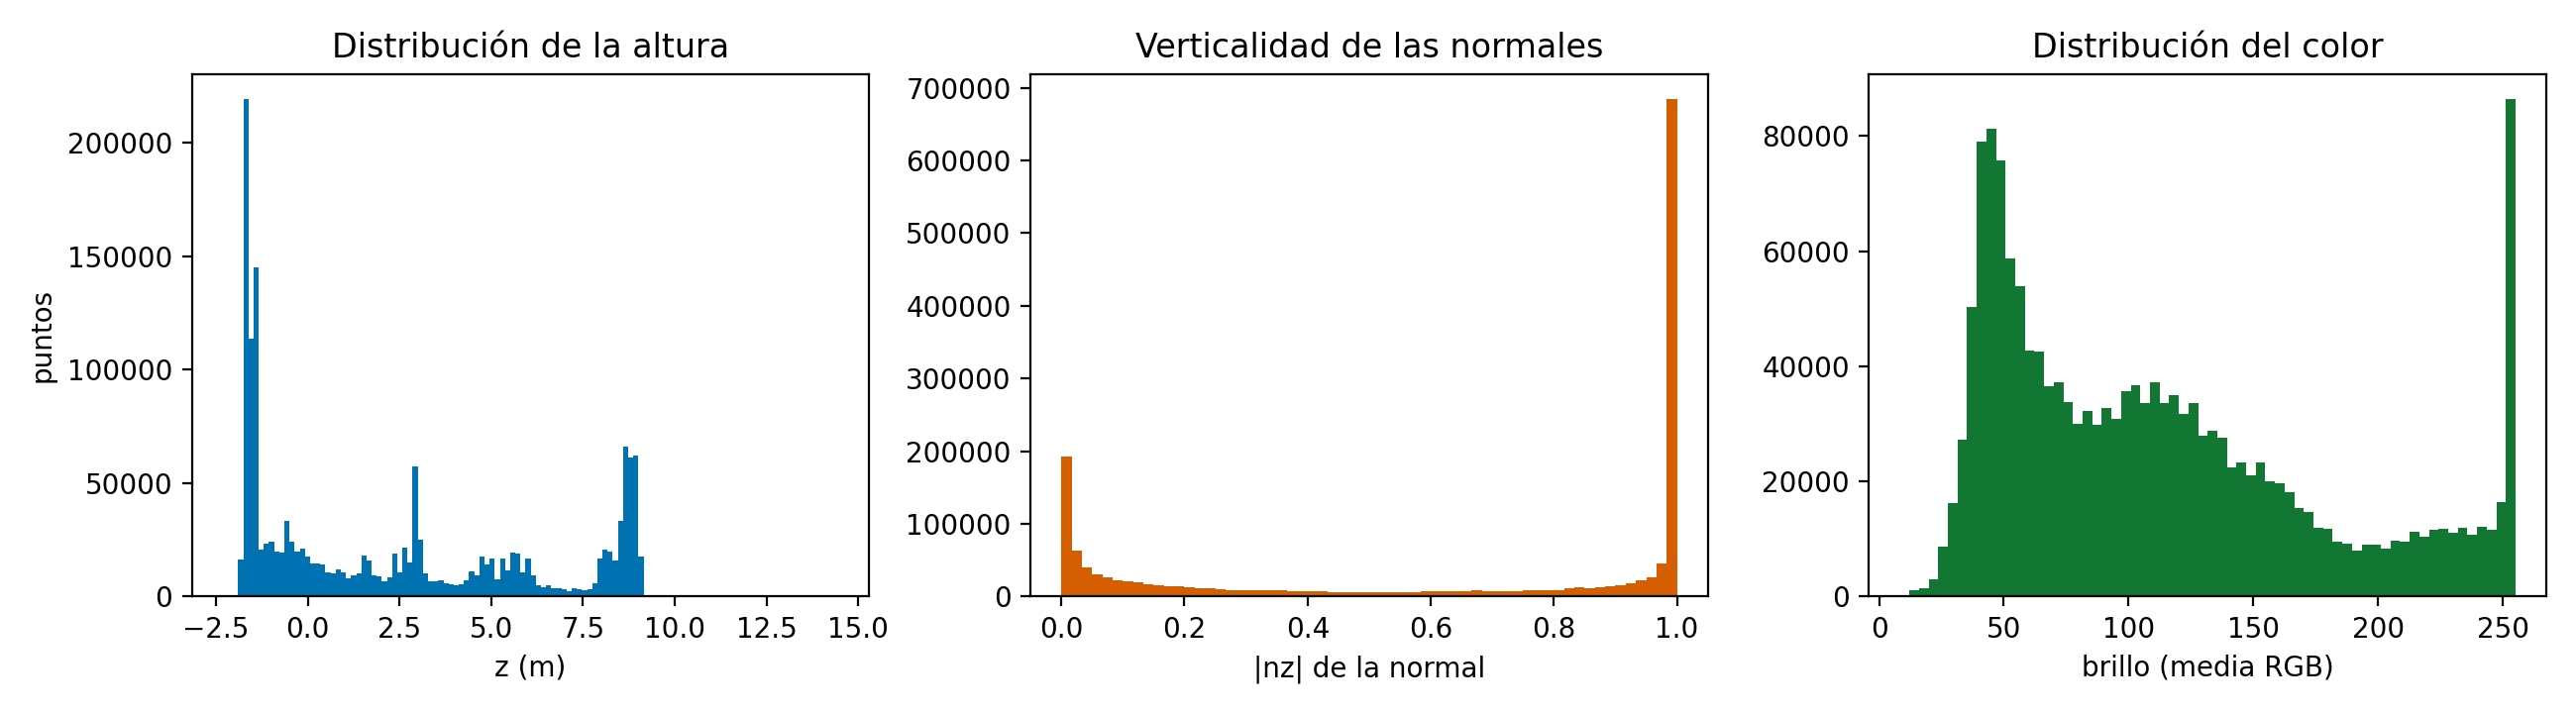
\includegraphics[width=\linewidth]{figures/fig1.png}
\caption{Histogramas de altura, normales y color de la nube original.}
\end{figure}
\begin{figure}[H]
\centering
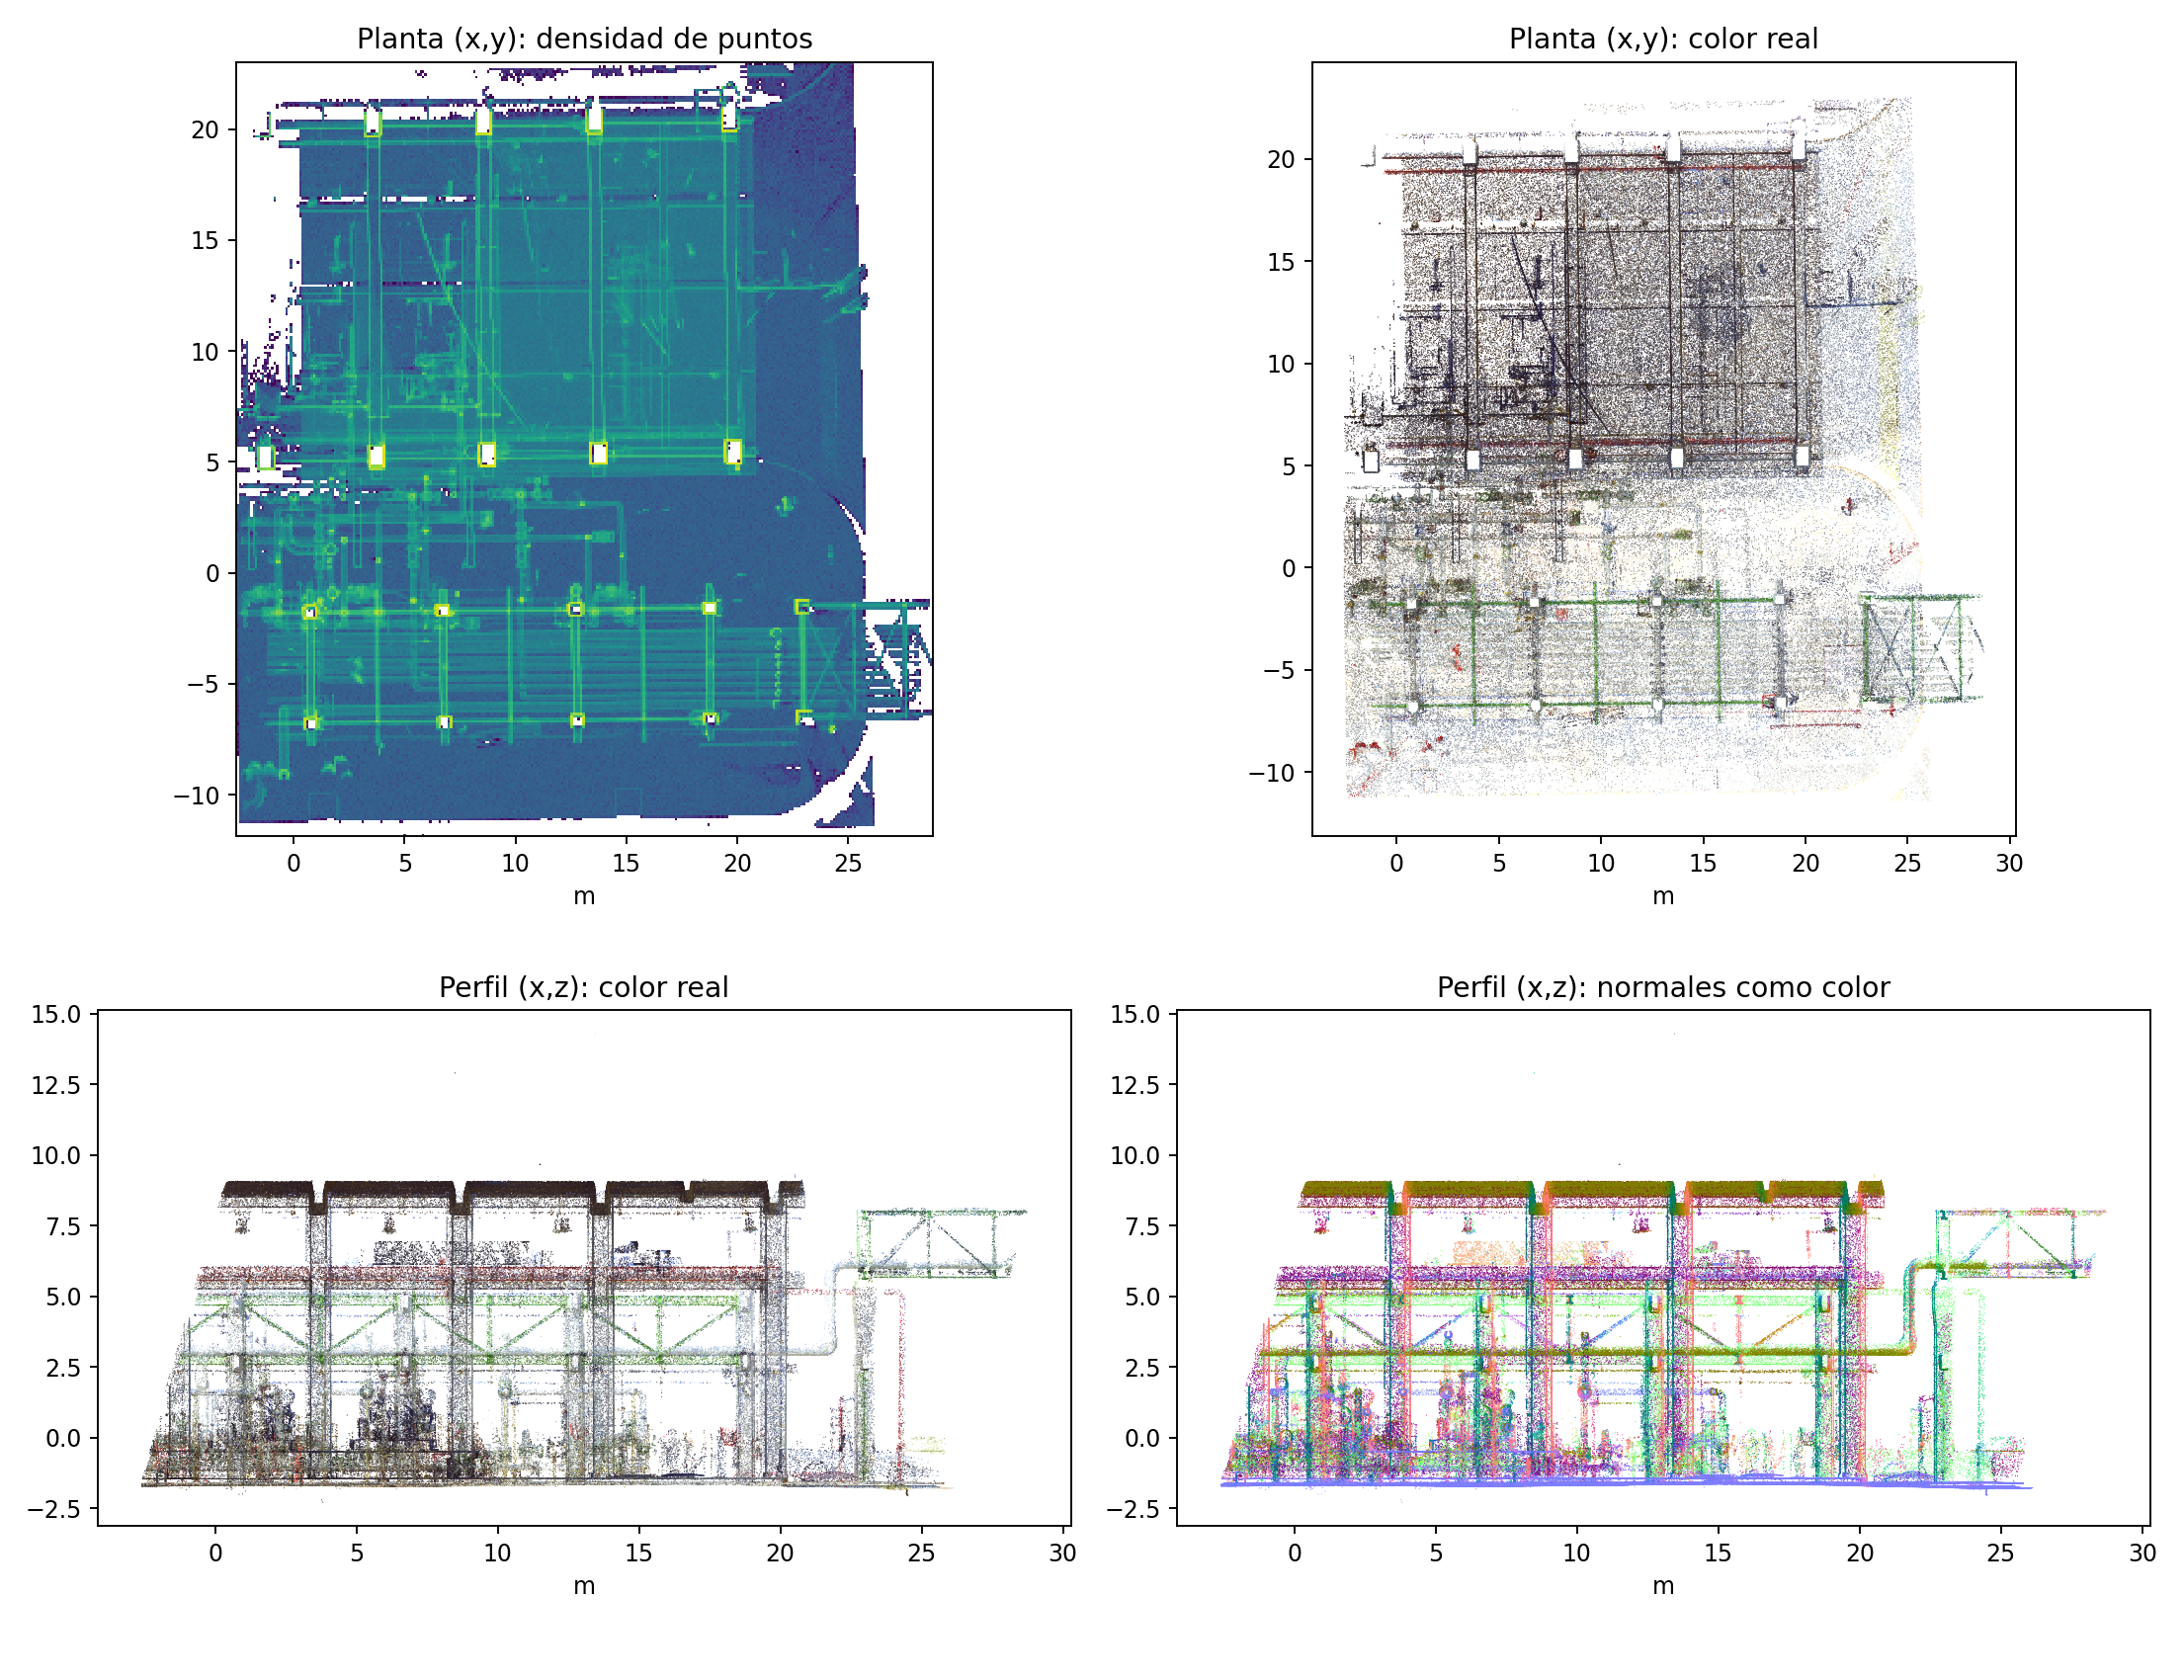
\includegraphics[width=0.85\linewidth]{figures/fig2.png}
\caption{Vistas en planta y de perfil de la nube original.}
\end{figure}

\paragraph{Submuestreo por voxel.} Cada celda de la grilla se reemplaza por el promedio de posición y color y por la normal promedio renormalizada, y se guarda la correspondencia punto original $\to$ voxel para propagar etiquetas al final. Tamaños probados en la exploración:

\begin{table}[H]
\centering
\begin{tabular}{lrr}
\toprule
Voxel & Puntos restantes & \% del original \\
\midrule
0,03 m & 1\,629\,452 & 98,9 \\
0,05 m & 1\,041\,806 & 63,3 \\
0,08 m (exploración) & 459\,991 & 27,9 \\
0,10 m & 305\,071 & 18,5 \\
0,15 m & 142\,839 & 8,7 \\
\bottomrule
\end{tabular}
\caption{Reducción de la nube según el tamaño de voxel.}
\end{table}

El pipeline de segmentación usa dos resoluciones: una nube global con voxel de 0,10~m (305\,071 puntos), sobre la que se ejecutan RANSAC, el clustering y la clasificación, y una nube de detalle con voxel de 0,05~m (1\,041\,806 puntos). La exploración del Rol~1 usó 0,08~m para elegir el compromiso entre tamaño y conservación de elementos delgados.

\paragraph{Limpieza y variables.} En la exploración se descartaron los voxeles con menos de 4 vecinos en un radio de 0,25~m (1\,006 voxeles, el 0,22\,\%), con lo que quedaron 458\,985 puntos. Cada punto se describe con 13 variables: posición, normal y $|n_z|$, color normalizado y tres medidas de forma local obtenidas por PCA sobre los 20 vecinos más cercanos, a partir de los autovalores $\lambda_1\ge\lambda_2\ge\lambda_3$ de la covarianza local:
\[
\text{linealidad}=\frac{\lambda_1-\lambda_2}{\lambda_1},\qquad
\text{planaridad}=\frac{\lambda_2-\lambda_3}{\lambda_1},\qquad
\text{esfericidad}=\frac{\lambda_3}{\lambda_1}.
\]
La linealidad es alta en tuberías y vigas, la planaridad en pisos, techos y paredes, y la esfericidad en volúmenes y ruido. Las variables se estandarizan porque están en unidades distintas y el clustering se basa en distancias.

\paragraph{Propagación de etiquetas.} La etiqueta de cada punto original es la de su voxel; los puntos cuyo voxel fue descartado como ruido quedan sin etiqueta. En una prueba con una etiqueta artificial ($z$ mayor o menor que 3~m), la etiqueta propagada coincidió con la directa en el 99,59\,\% de los puntos.

\begin{figure}[H]
\centering
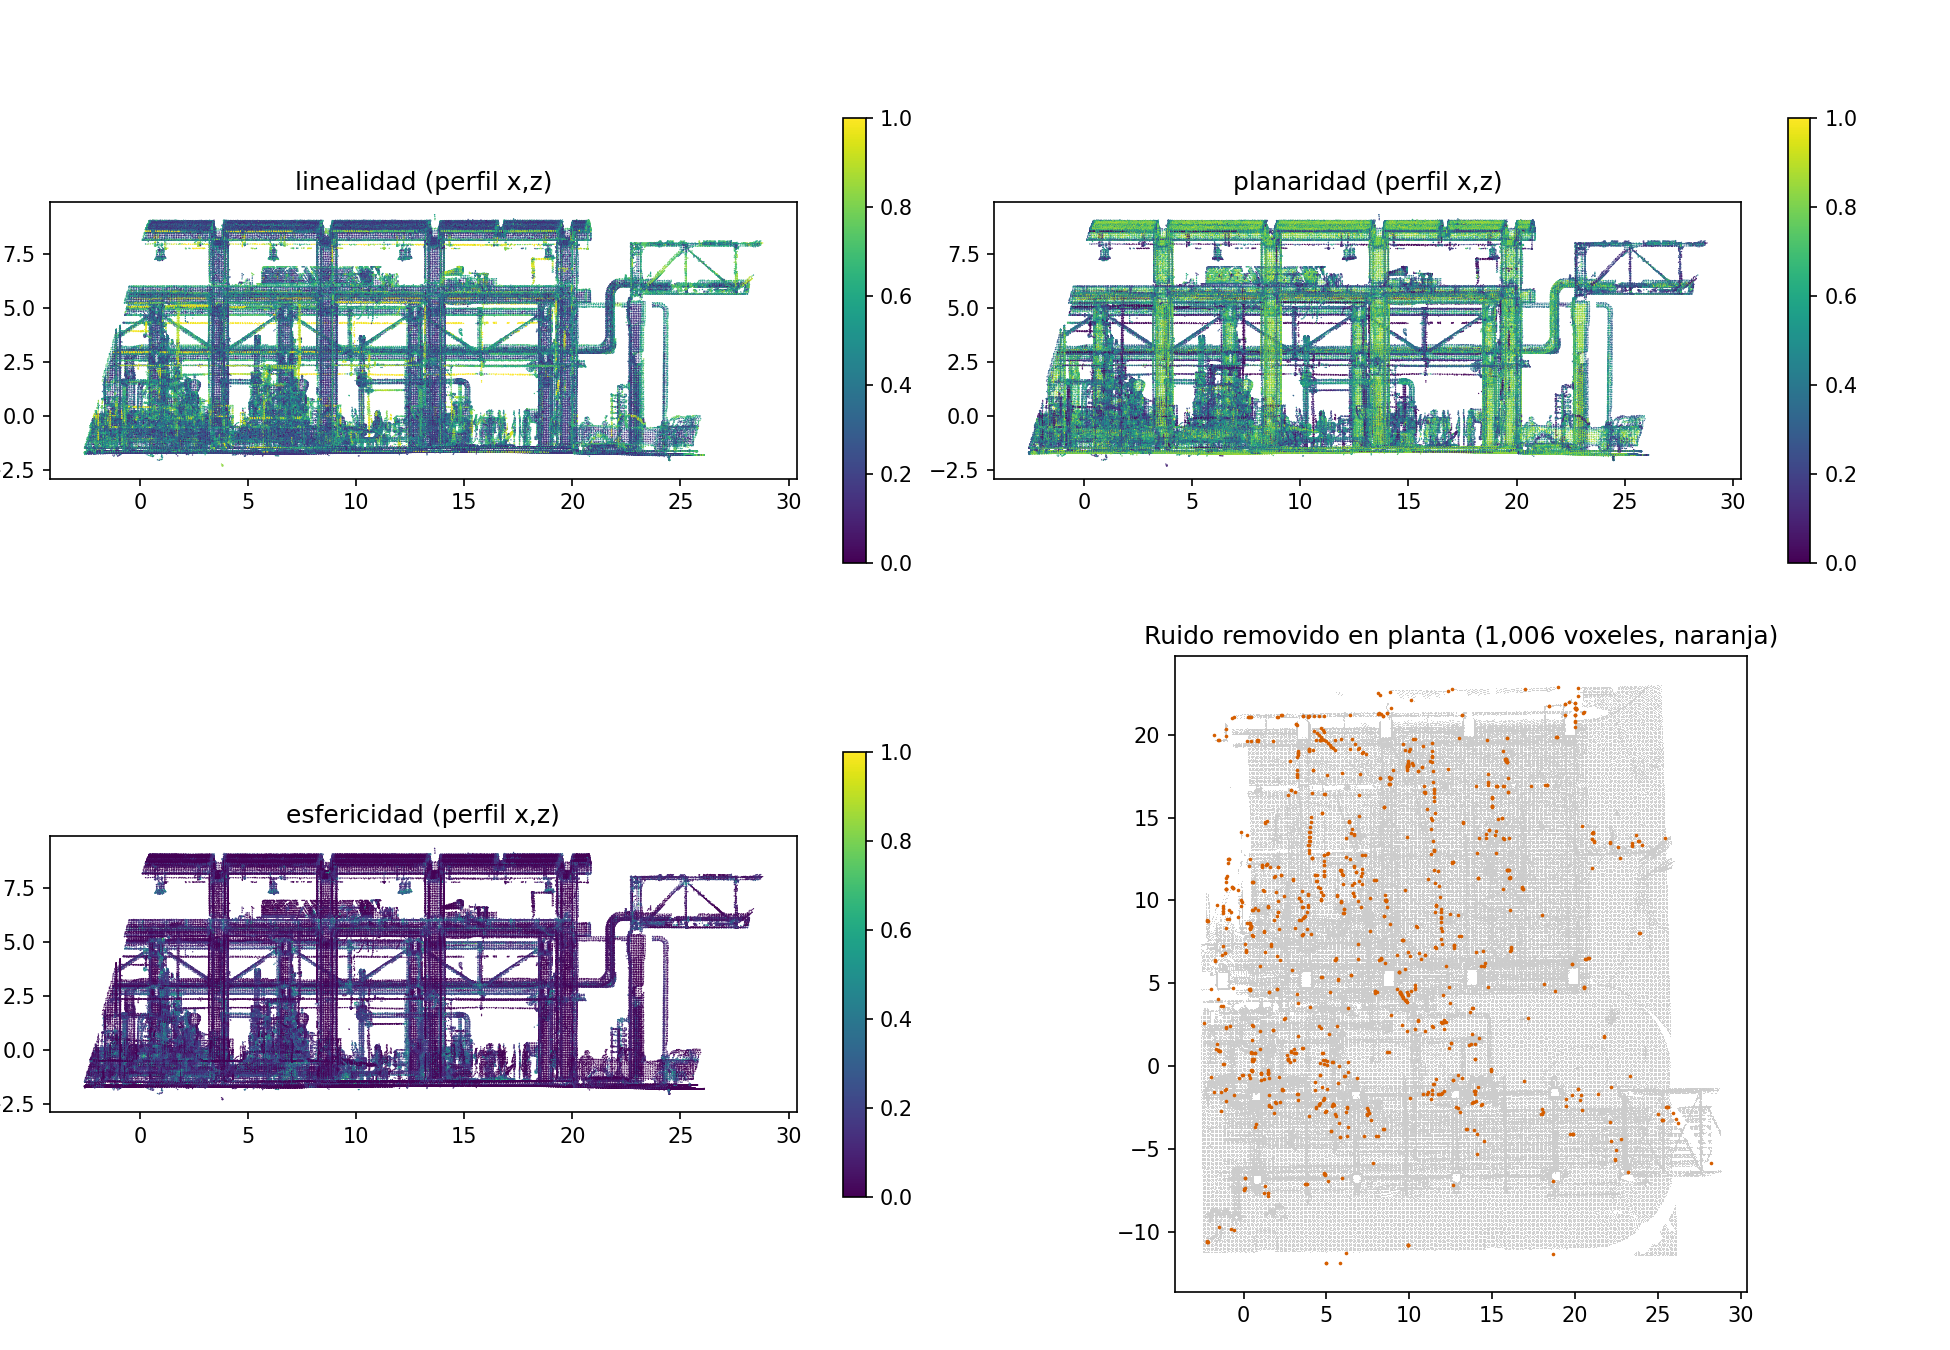
\includegraphics[width=0.85\linewidth]{figures/fig3.png}
\caption{Variables locales de forma (linealidad, planaridad, esfericidad) y puntos eliminados como ruido.}
\end{figure}

\section{Etapa 1: estructura global}
\textit{Responsable: Josué Yeremi Huamán Huamaní (Rol 2).}

La primera etapa separa las superficies planas grandes con RANSAC iterativo sobre la nube global. Se extrae un plano a la vez y se retiran sus puntos antes de buscar el siguiente. Parámetros: distancia máxima al plano 0,05~m, 500 iteraciones, mínimo 3\,000 puntos por plano, hasta 6 planos, semilla 42. Con la nube global, los 6 planos encontrados agrupan 83\,004 puntos (el 27,2\,\% de la nube global) y todos son horizontales (normal casi igual a $(0,0,1)$):

\begin{table}[H]
\centering
\begin{tabular}{rrrl}
\toprule
Plano & Altura $z$ (m) & Puntos (global) & Interpretación \\
\midrule
0 & $-1{,}70$ & 39\,852 & Piso \\
1 & $-1{,}66$ & 18\,041 & Piso (nivel muy próximo al anterior) \\
2 & $-0{,}45$ & 7\,082 & Plano horizontal bajo \\
4 & $-0{,}92$ & 6\,326 & Plano horizontal bajo \\
3 & 8,22 & 6\,482 & Plano horizontal alto \\
5 & 9,07 & 5\,221 & Techo ($z$ cercana a 9~m) \\
\bottomrule
\end{tabular}
\caption{Planos detectados por RANSAC en la nube global.}
\end{table}

RANSAC solo reconoce que un conjunto de puntos es plano; no decide si es piso, techo o plataforma. Esa decisión se toma después con la altura relativa de cada región respecto a la escena. No se detectaron planos verticales con este criterio: las paredes aparecen en una proporción muy baja (0,6\,\%) porque la fábrica es sobre todo estructura abierta de columnas y vigas. El eje vertical se asume igual a $z$, hipótesis consistente con los histogramas de la sección~2 pero no confirmada con una referencia externa.

\paragraph{Decisión de diseño.} Los planos se extraen antes del clustering para que superficies de gran extensión no <<peguen>> entre sí a elementos delgados cercanos. Los puntos que no pertenecen a ningún plano (222\,067 de la nube global) pasan a la etapa 2.

\section{Etapa 2: objetos}
\textit{Responsable: Enrique Zheng Chan (Rol 3).}

\paragraph{Agrupamiento espacial.} Sobre los puntos restantes se aplica un agrupamiento por conectividad de vecindad, equivalente a DBSCAN con vecindarios acotados a los 64 vecinos más próximos (radio $\varepsilon=0{,}25$~m, mínimo 8 puntos por núcleo, tamaño de segmento entre 30 y 100\,000 puntos). Es una aproximación de DBSCAN que limita la memoria y no es DBSCAN exacto; el repositorio incluye además una versión exacta por radio para recortes de hasta 20\,000 puntos. Con la nube global se obtienen 65 clusters (tamaño mediano de 100 puntos), con una cobertura geométrica del 33,6\,\% de los puntos originales.

\paragraph{Un hallazgo importante: el componente gigante.}
% VERIFICAR con Enrique: 217 686 candidatos vs 222 067 puntos fuera de planos (diferencia de 4 381 puntos).
De los 217\,686 puntos candidatos al clustering, 201\,598 (el 92,6\,\% de los candidatos y el 66,1\,\% de la nube global) quedan conectados en un único componente, porque las columnas, vigas y tuberías de la estructura se tocan entre sí. Ese componente supera el tamaño máximo y se descarta, y por eso el clustering espacial por sí solo cubre poco. Esto motivó el refinamiento local descrito más abajo.

\paragraph{Descriptores de forma y clasificación por reglas.} A cada región se le calculan descriptores PCA (linealidad, planaridad, alineación del eje principal con la vertical, relación entre la extensión vertical y la horizontal, razón de la sección transversal y, para tuberías, la fracción de normales radiales y la cobertura angular). Con ellos se puntúan las clases mediante reglas interpretables, por ejemplo:
\begin{itemize}
\item \textbf{Piso / techo:} plano con normal alineada con la vertical ($\ge0{,}8$) y alta planaridad, ubicado en la parte baja (altura relativa $\le0{,}22$) o alta ($\ge0{,}78$) de la escena.
\item \textbf{Pared:} plano con normal casi horizontal y alta planaridad.
\item \textbf{Columna:} región alargada con eje principal vertical (alineación $\ge0{,}8$) y relación vertical/horizontal $\ge1{,}45$.
\item \textbf{Viga:} región con linealidad $\ge0{,}72$ y eje principal no vertical.
\item \textbf{Tubería:} región lineal con sección transversal casi circular y normales radiales respecto al eje.
\end{itemize}
Una clase se asigna solo si su puntaje es al menos 0,62 y supera al segundo en 0,12; en caso contrario la región queda como <<desconocido>>. Los puntajes son heurísticos, no probabilidades.

\paragraph{Refinamiento V3 por tiles.} Para dividir el componente gigante se parte la nube en baldosas de 2~m con un halo de 0,20~m. En cada baldosa se voxeliza a 0,20~m, se agrupan las celdas vecinas con normales compatibles (diferencia máxima de 35°) y se vuelve a calcular el descriptor y a aplicar las reglas. Se procesaron 637 baldosas; V3 aceptó 91\,300 puntos globales nuevos y conservó sin cambios los 39\,913 puntos ya etiquetados por V1.

\subsection{Comparación experimental de algoritmos de clustering}
\label{sec:comparacion}
\textit{Análisis complementario (Rol 1), script \texttt{scripts/04\_comparar\_clustering.py}.}

El pipeline de segmentación usa conectividad tipo DBSCAN y reglas. Para justificar esa decisión frente a los algoritmos vistos en clase, se compararon k-means, mezclas gaussianas (GMM, covarianza diagonal), clustering jerárquico (Ward) y DBSCAN sobre las variables estandarizadas del preprocesamiento (nube de 458\,985 puntos). Por costo, cada algoritmo se ejecutó sobre muestras aleatorias de 10\,000 puntos (3 semillas: 0, 1 y 2); k varía de 2 a 10 y DBSCAN usa $\min\text{\_}samples=10$ con $\varepsilon\in\{0{,}5;\,0{,}75;\,1;\,1{,}5;\,2\}$ en el espacio estandarizado. Las métricas son la silhouette (mayor es mejor, entre $-1$ y 1) y el índice de Davies-Bouldin (menor es mejor). Se probaron dos conjuntos de variables: las 13 completas y 10 sin la posición $(x,y,z)$.

\begin{table}[H]
\centering
\small
\begin{tabular}{llrrrr}
\toprule
Variables & Algoritmo & Mejor $k$ & Silhouette & Davies-B. & Tiempo (s) \\
\midrule
13 (con posición) & k-means & 9 & $0{,}208\pm0{,}002$ & 1,65 & 0,1 \\
 & GMM (diag.) & 2 & $0{,}165\pm0{,}003$ & 2,08 & 0,1 \\
 & Ward & 5 & $0{,}170\pm0{,}004$ & 2,12 & 3,3 \\
\midrule
10 (sin posición) & k-means & 10 & $0{,}276\pm0{,}003$ & 1,33 & 0,1 \\
 & GMM (diag.) & 2 & $0{,}154\pm0{,}042$ & 1,95 & 0,1 \\
 & Ward & 10 & $0{,}204\pm0{,}008$ & 1,62 & 3,5 \\
\bottomrule
\end{tabular}
\caption{Mejor $k$ por silhouette (media $\pm$ desviación estándar en 3 muestras de 10\,000 puntos). El tiempo es por ajuste, con $n=10\,000$.}
\end{table}

\begin{table}[H]
\centering
\small
\begin{tabular}{rrrrrrr}
\toprule
& \multicolumn{3}{c}{13 variables} & \multicolumn{3}{c}{10 variables (sin posición)} \\
\cmidrule(lr){2-4}\cmidrule(lr){5-7}
$\varepsilon$ & Clusters & Ruido (\%) & Silh. & Clusters & Ruido (\%) & Silh. \\
\midrule
0,5 & 5,0 & 75 & 0,113 & 18,3 & 61 & 0,340 \\
0,75 & 12,0 & 67 & 0,329 & 14,3 & 42 & 0,161 \\
1,0 & 22,0 & 53 & 0,149 & 8,7 & 20 & $-0{,}051$ \\
1,5 & 9,0 & 19 & $-0{,}119$ & 1,0 & 2 & n.d. \\
2,0 & 1,3 & 2 & 0,100 & 1,0 & 0 & n.d. \\
\bottomrule
\end{tabular}
\caption{DBSCAN sobre las variables estandarizadas (promedio de 3 muestras). La silhouette se calcula sin los puntos de ruido y no está definida con un solo cluster (n.d.).}
\end{table}

\begin{figure}[H]
\centering
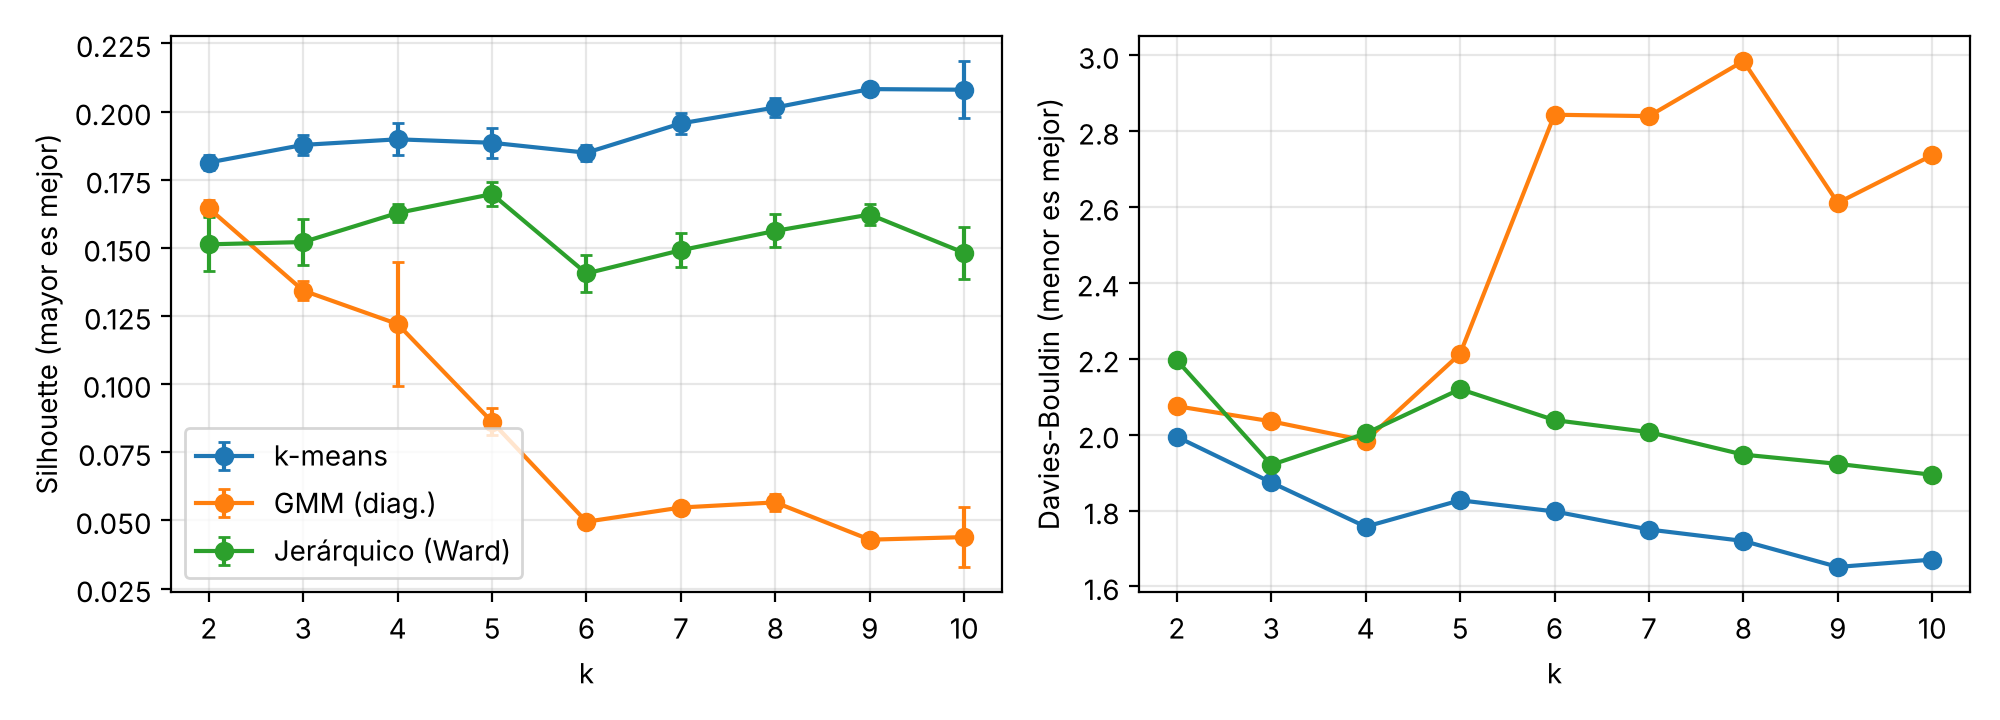
\includegraphics[width=\linewidth]{figures/cl_silhouette_vs_k.png}
\caption{Silhouette y Davies-Bouldin en función de $k$ con las 13 variables (barras: desviación estándar entre muestras).}
\end{figure}

\begin{figure}[H]
\centering
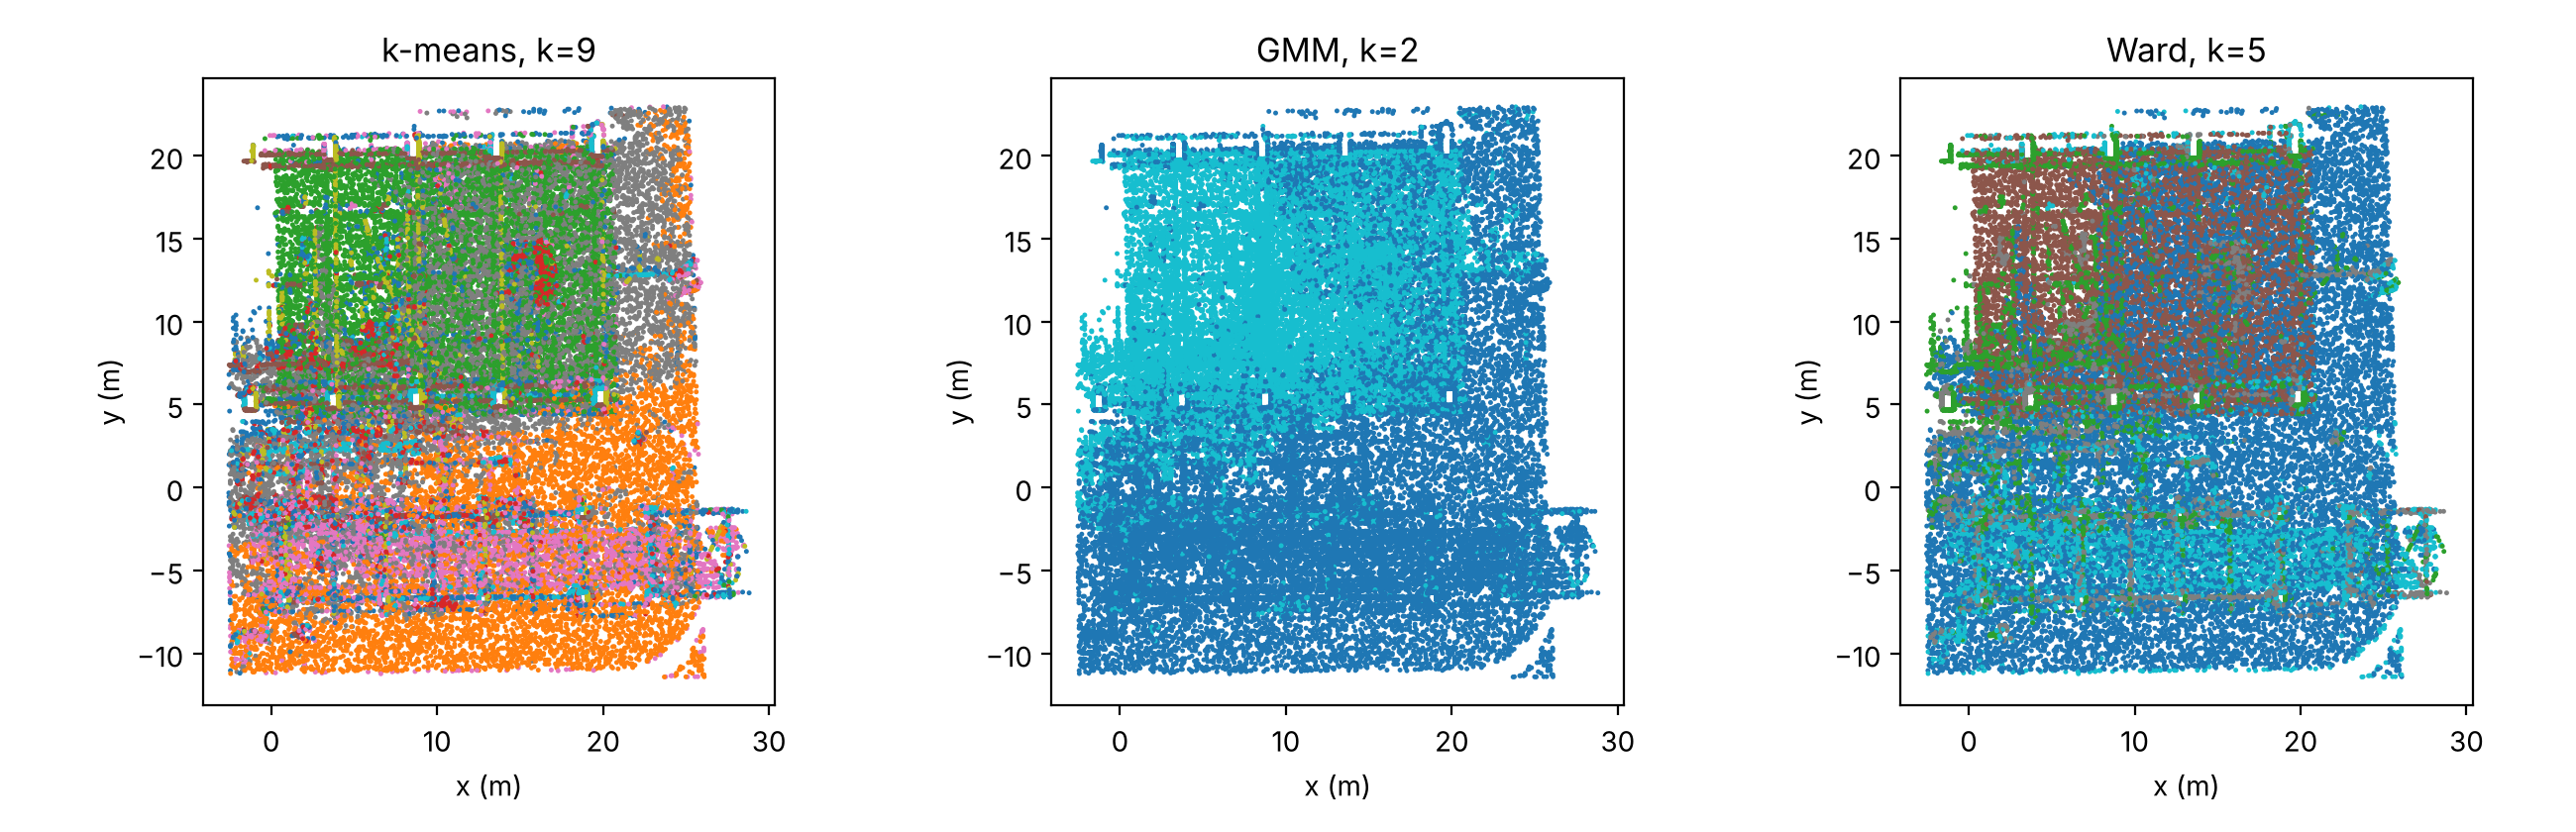
\includegraphics[width=\linewidth]{figures/cl_planta_con_pos.png}
\caption{Planta XY coloreada por cluster con las 13 variables (60\,000 puntos; mejor $k$ de cada algoritmo).}
\label{fig:conpos}
\end{figure}

\begin{figure}[H]
\centering
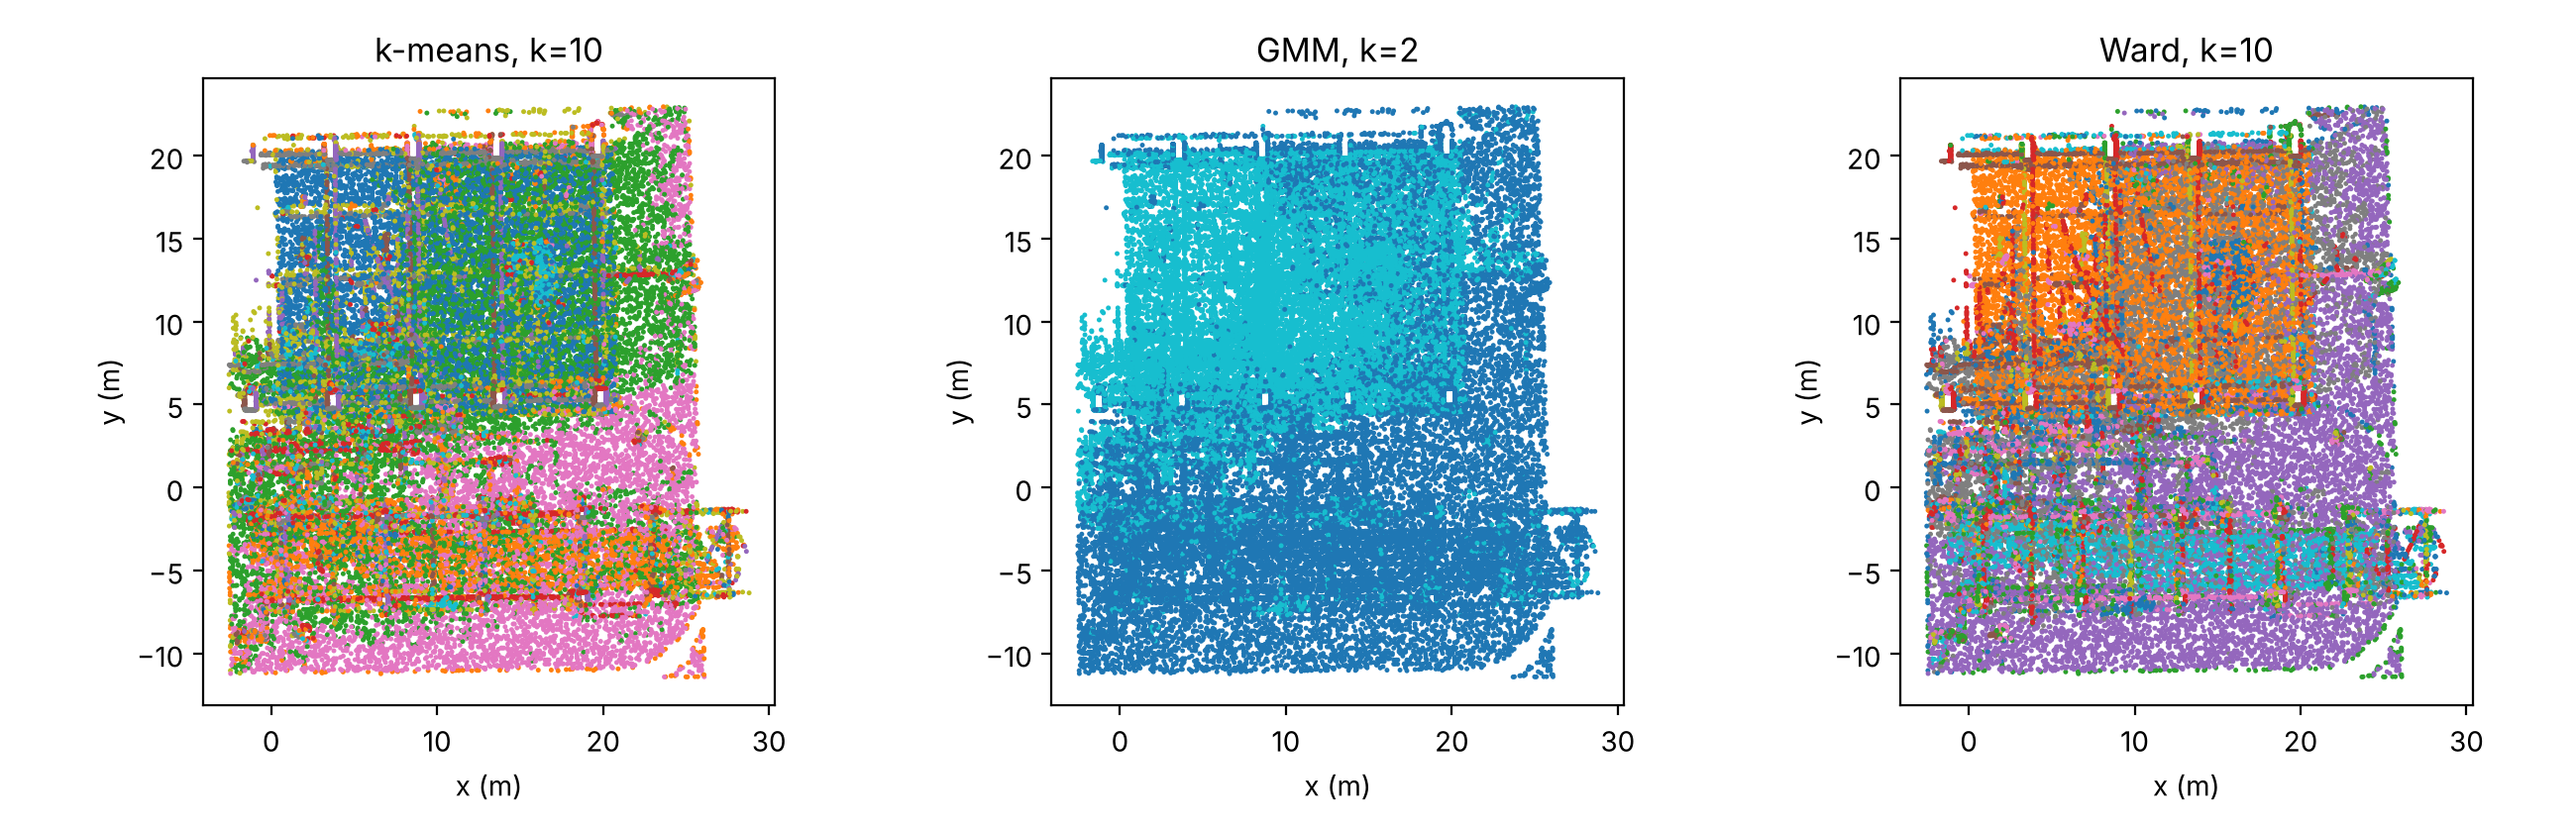
\includegraphics[width=\linewidth]{figures/cl_planta_sin_pos.png}
\caption{Planta XY coloreada por cluster sin usar la posición como variable (10 variables).}
\end{figure}

\paragraph{Lectura de los resultados.}
\begin{itemize}
\item Ninguna configuración separa grupos bien definidos: las silhouettes están entre 0,04 y 0,28, y la mejor es k-means con 10 variables (0,276). Los datos forman un continuo más que clusters compactos.
\item Con las 13 variables, la posición domina: la planta (Figura~\ref{fig:conpos}) muestra que los clusters son zonas del espacio y no objetos, de modo que un k-means sobre todo el conjunto reparte la fábrica en regiones. Quitar $(x,y,z)$ sube la silhouette de k-means de 0,208 a 0,276 y hace que los grupos dependan de la forma local, la normal y el color.
\item Los perfiles medios de los 10 clusters de k-means sin posición son interpretables. Por ejemplo, hay grupos de superficies planas horizontales ($|n_z|\approx0{,}95$--0,99, planaridad $\approx0{,}74$--0,79) oscuras y claras, grupos de superficies planas verticales ($|n_z|<0{,}25$), un grupo con linealidad alta ($0{,}65$) típico de elementos alargados, y uno con esfericidad alta ($0{,}41$) típico de volúmenes o ruido. Es una lectura de los promedios, no una validación contra etiquetas reales.
\item Las mezclas gaussianas con covarianza diagonal tienen su mejor silhouette en $k=2$ y empeoran al crecer $k$, y su Davies-Bouldin sube de forma marcada: los grupos no se aproximan bien por gaussianas.
\item Ward da resultados intermedios, pero su costo crece con $n^2$; con 10\,000 puntos ya es 30 veces más lento que k-means y no escala a los 458\,985 puntos.
\item DBSCAN tiene silhouettes altas en algunos $\varepsilon$ (0,329 con $\varepsilon=0{,}75$), pero marca como ruido entre el 42\,\% y el 75\,\% de los puntos en esos casos, y con $\varepsilon$ grandes colapsa en un único cluster. La silhouette se mide solo sobre los puntos no ruidosos, por lo que esos valores no son comparables con los de los demás algoritmos. Esto coincide con el hallazgo del componente gigante (sección~4) y es una razón para segmentar por etapas con RANSAC, clustering espacial y reglas, en lugar de un único clustering global sobre todas las variables.
\end{itemize}

\paragraph{Limitaciones del experimento.} Se usaron muestras de 10\,000 puntos (2,2\,\% de la nube), la silhouette es una medida interna que no evalúa si un cluster corresponde a una clase real, y no hay etiquetas para calcular ARI o IoU. Los clusters no se transfirieron al PLY final: la segmentación entregada es la del pipeline por reglas (secciones 3--6). Este análisis sirve para comparar algoritmos y justificar el diseño, no para medir la calidad de la segmentación.

\section{Integración y exportación}
\label{sec:integracion}
\textit{Responsable: Requelmy Limaco Porras (Rol 4).}

Las etapas se unieron en un único script reproducible, \texttt{scripts/run\_pipeline.py}, que ejecuta en orden: preprocesamiento por voxel, planos RANSAC y clustering, clasificación por reglas (V1), análisis del componente gigante y refinamiento V3. Con semilla 42, el pipeline completo se ejecutó en 50,8~s sobre la nube de la actividad. Uso:
\begin{quote}\small\ttfamily\raggedright
uv run python scripts/run\_pipeline.py \\ --input data/raw/FARO\_Scan\_Full\_Sub1\_down3\_with\_normals.ply
\end{quote}
Las etiquetas de la nube global se propagan a los 1\,647\,021 puntos originales por pertenencia al voxel, y se exporta el PLY con un color fijo por clase:

\begin{table}[H]
\centering
\begin{tabular}{llll}
\toprule
Clase & Color & Clase & Color \\
\midrule
Piso (\textit{floor}) & verde & Viga (\textit{beam}) & morado \\
Techo (\textit{ceiling}) & amarillo & Tubería (\textit{pipe}) & cian \\
Pared (\textit{wall}) & azul & Otro (\textit{other}) & naranja \\
Columna (\textit{column}) & rojo & Desconocido (\textit{unknown}) & gris \\
\bottomrule
\end{tabular}
\caption{Color asignado a cada clase en el PLY exportado.}
\end{table}

\paragraph{Corrección realizada durante la integración.} Al ejecutar el código sobre la nube real, el techo salía con 0\,\% de los puntos. La causa era que la altura relativa de cada región se calculaba con el máximo de $z$ de la nube: unos 14 puntos aislados llegan a $z=14{,}5$~m, mientras que el techo real está cerca de 9~m, por lo que su altura relativa nunca alcanzaba el umbral de 0,78. Se cambió el límite de la escena para usar los percentiles 0,1 y 99,9 de las coordenadas, en \texttt{classify\_cloud.py} y \texttt{semantic\_v3.py}. Con este cambio el techo pasa de 0\,\% a 9,5\,\% y los puntos desconocidos bajan del 65,4\,\% al 57,2\,\%. Los puntos ya clasificados por V1 se conservaron.

\section{Resultados y evaluación}
\label{sec:resultados}
La tabla resume la clasificación final (V3) sobre los 1\,647\,021 puntos originales, y la comparación con V1:

\begin{table}[H]
\centering
\begin{tabular}{lrr}
\toprule
Clase & Puntos & \% \\
\midrule
Piso & 134\,991 & 8,2 \\
Techo & 155\,897 & 9,5 \\
Pared & 9\,769 & 0,6 \\
Columna & 124\,893 & 7,6 \\
Viga & 247\,040 & 15,0 \\
Tubería & 26\,582 & 1,6 \\
Otro & 5\,845 & 0,4 \\
Desconocido & 942\,004 & 57,2 \\
\midrule
Total & 1\,647\,021 & 100,0 \\
\bottomrule
\end{tabular}
\caption{Clasificación final (V3) de los puntos originales. Los porcentajes están redondeados a un decimal.}
\end{table}

\begin{table}[H]
\centering
\begin{tabular}{lrr}
\toprule
Etapa & Con clase (\%) & Desconocido (\%) \\
\midrule
V1 (planos + clustering + reglas) & 12,8 & 87,2 \\
V3 (refinamiento por tiles) & 42,8 & 57,2 \\
\bottomrule
\end{tabular}
\caption{Cobertura de clases en V1 y V3.}
\end{table}

V3 añadió 494\,260 puntos originales a los de V1. Estas cifras miden la cobertura de las reglas, no la calidad: no hay anotaciones humanas, por lo que no se calculan exactitud, precisión, recall ni IoU. Tampoco se ha demostrado que V3 sea más correcto que V1; solo que clasifica más puntos.

\paragraph{Evaluación cualitativa.} Con las vistas de la Figura~\ref{fig:v3} se observa que:
\begin{itemize}
\item Las columnas (rojo) aparecen en los nodos de la grilla regular de la planta y a lo largo de las alturas en los cortes, de acuerdo con la estructura real.
\item Las vigas (morado) siguen las líneas horizontales de los pórticos y de los racks a distintos niveles.
\item El techo (amarillo) se ubica a $z$ cercana a 9~m, en la parte norte y central de la planta; el piso (verde) se reconoce solo en parte, sobre todo hacia el sur.
\item Gran parte del equipo de proceso (tuberías densas, válvulas, bombas) y buena parte del piso interior quedan en gris. Es donde el componente gigante y los umbrales fijos pesan más.
\end{itemize}

\begin{figure}[H]
\centering
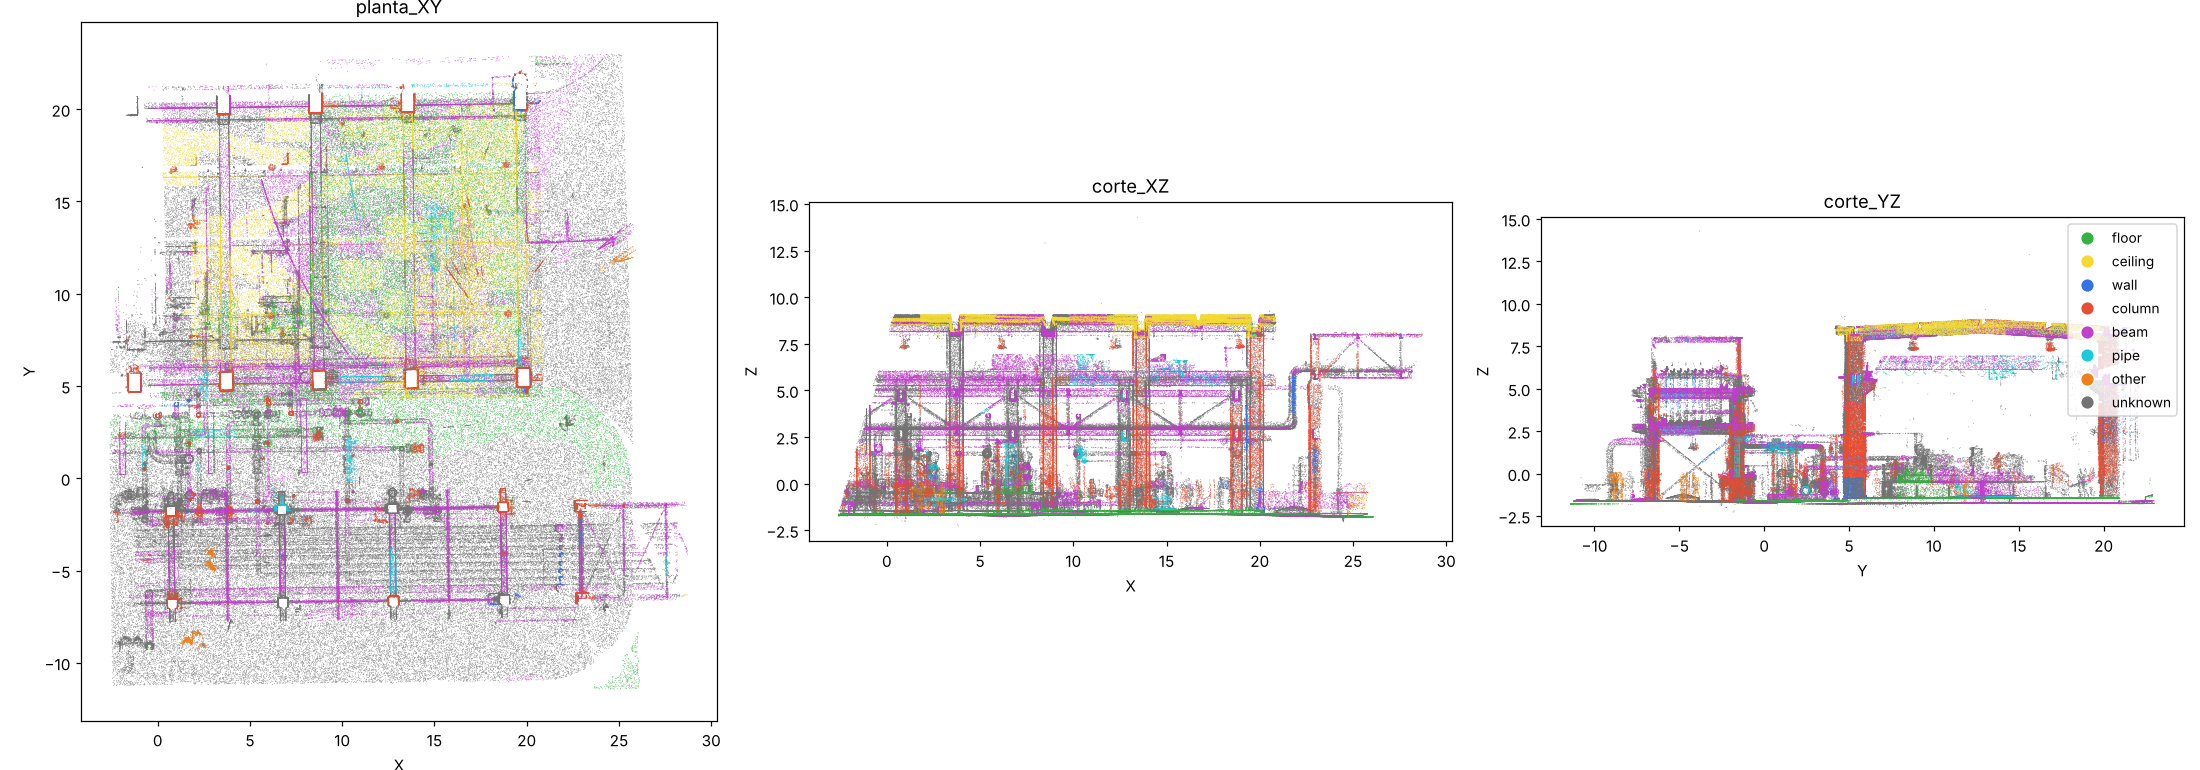
\includegraphics[width=\linewidth]{figures/fig4.png}
\caption{Resultado final (V3): planta (XY) y cortes XZ e YZ, con una muestra de 400\,000 puntos. Gris = desconocido.}
\label{fig:v3}
\end{figure}
\begin{figure}[H]
\centering
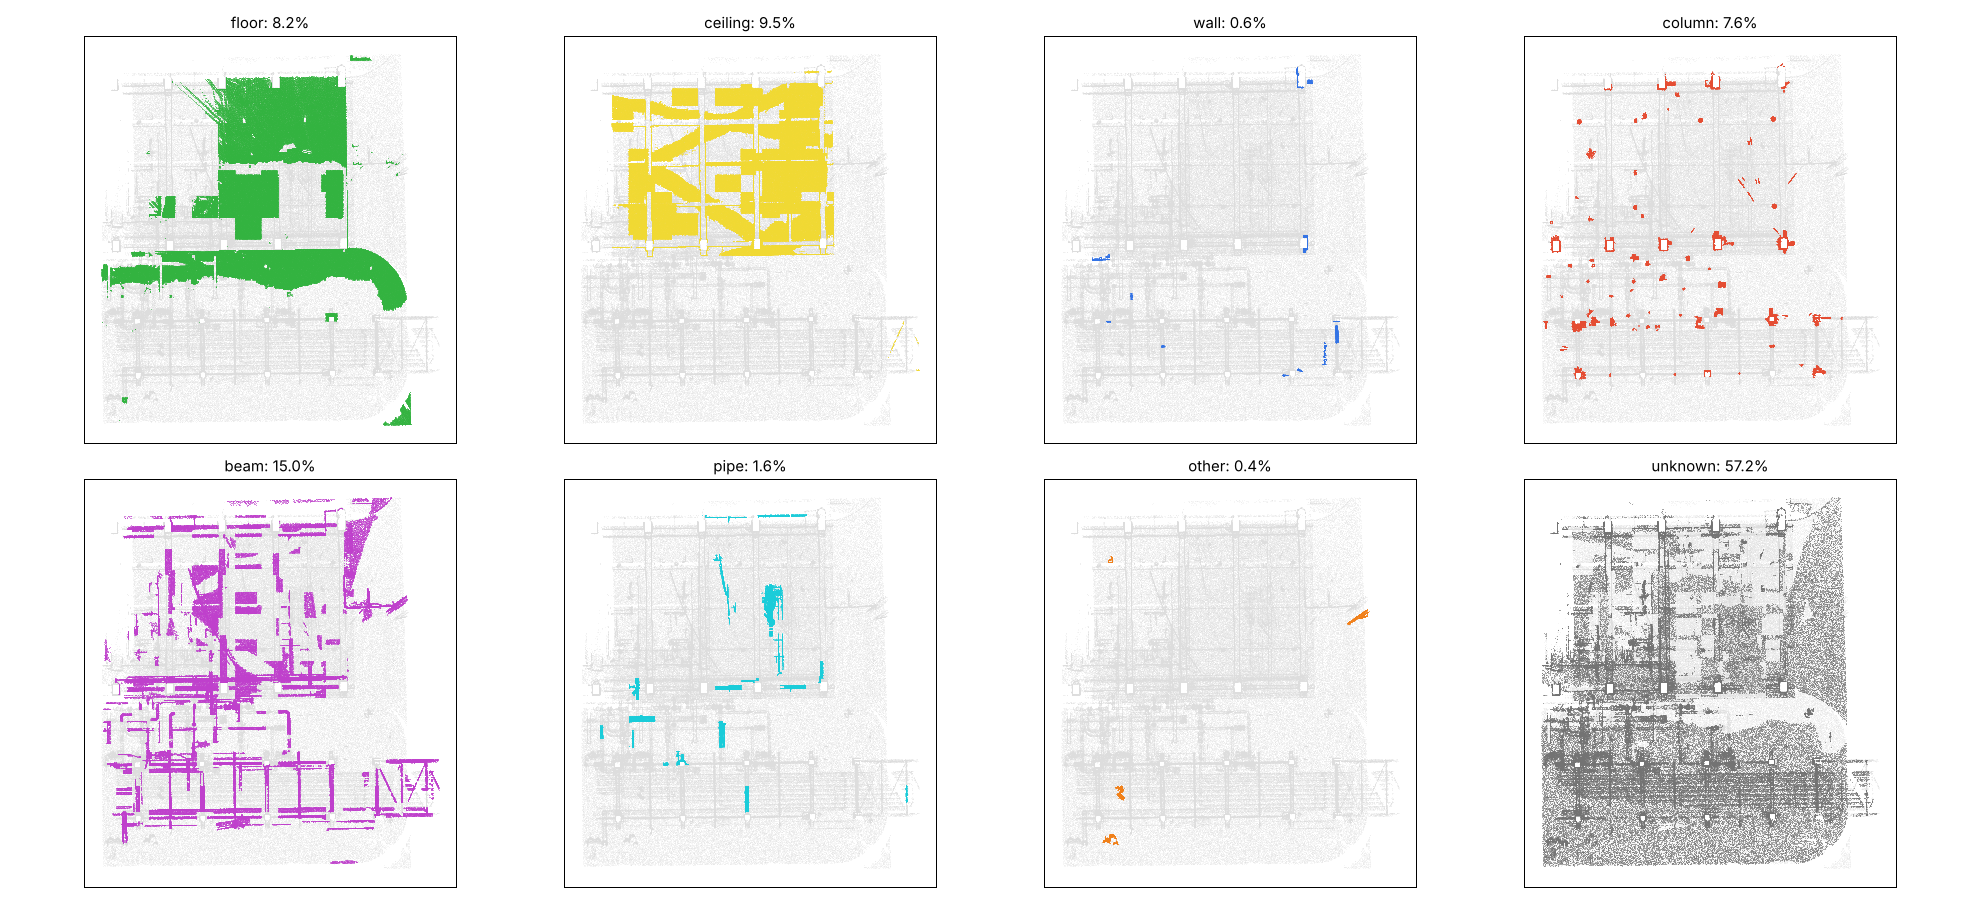
\includegraphics[width=\linewidth]{figures/fig5.png}
\caption{Cada clase resaltada sobre la planta, con su porcentaje de puntos.}
\end{figure}
\begin{figure}[H]
\centering
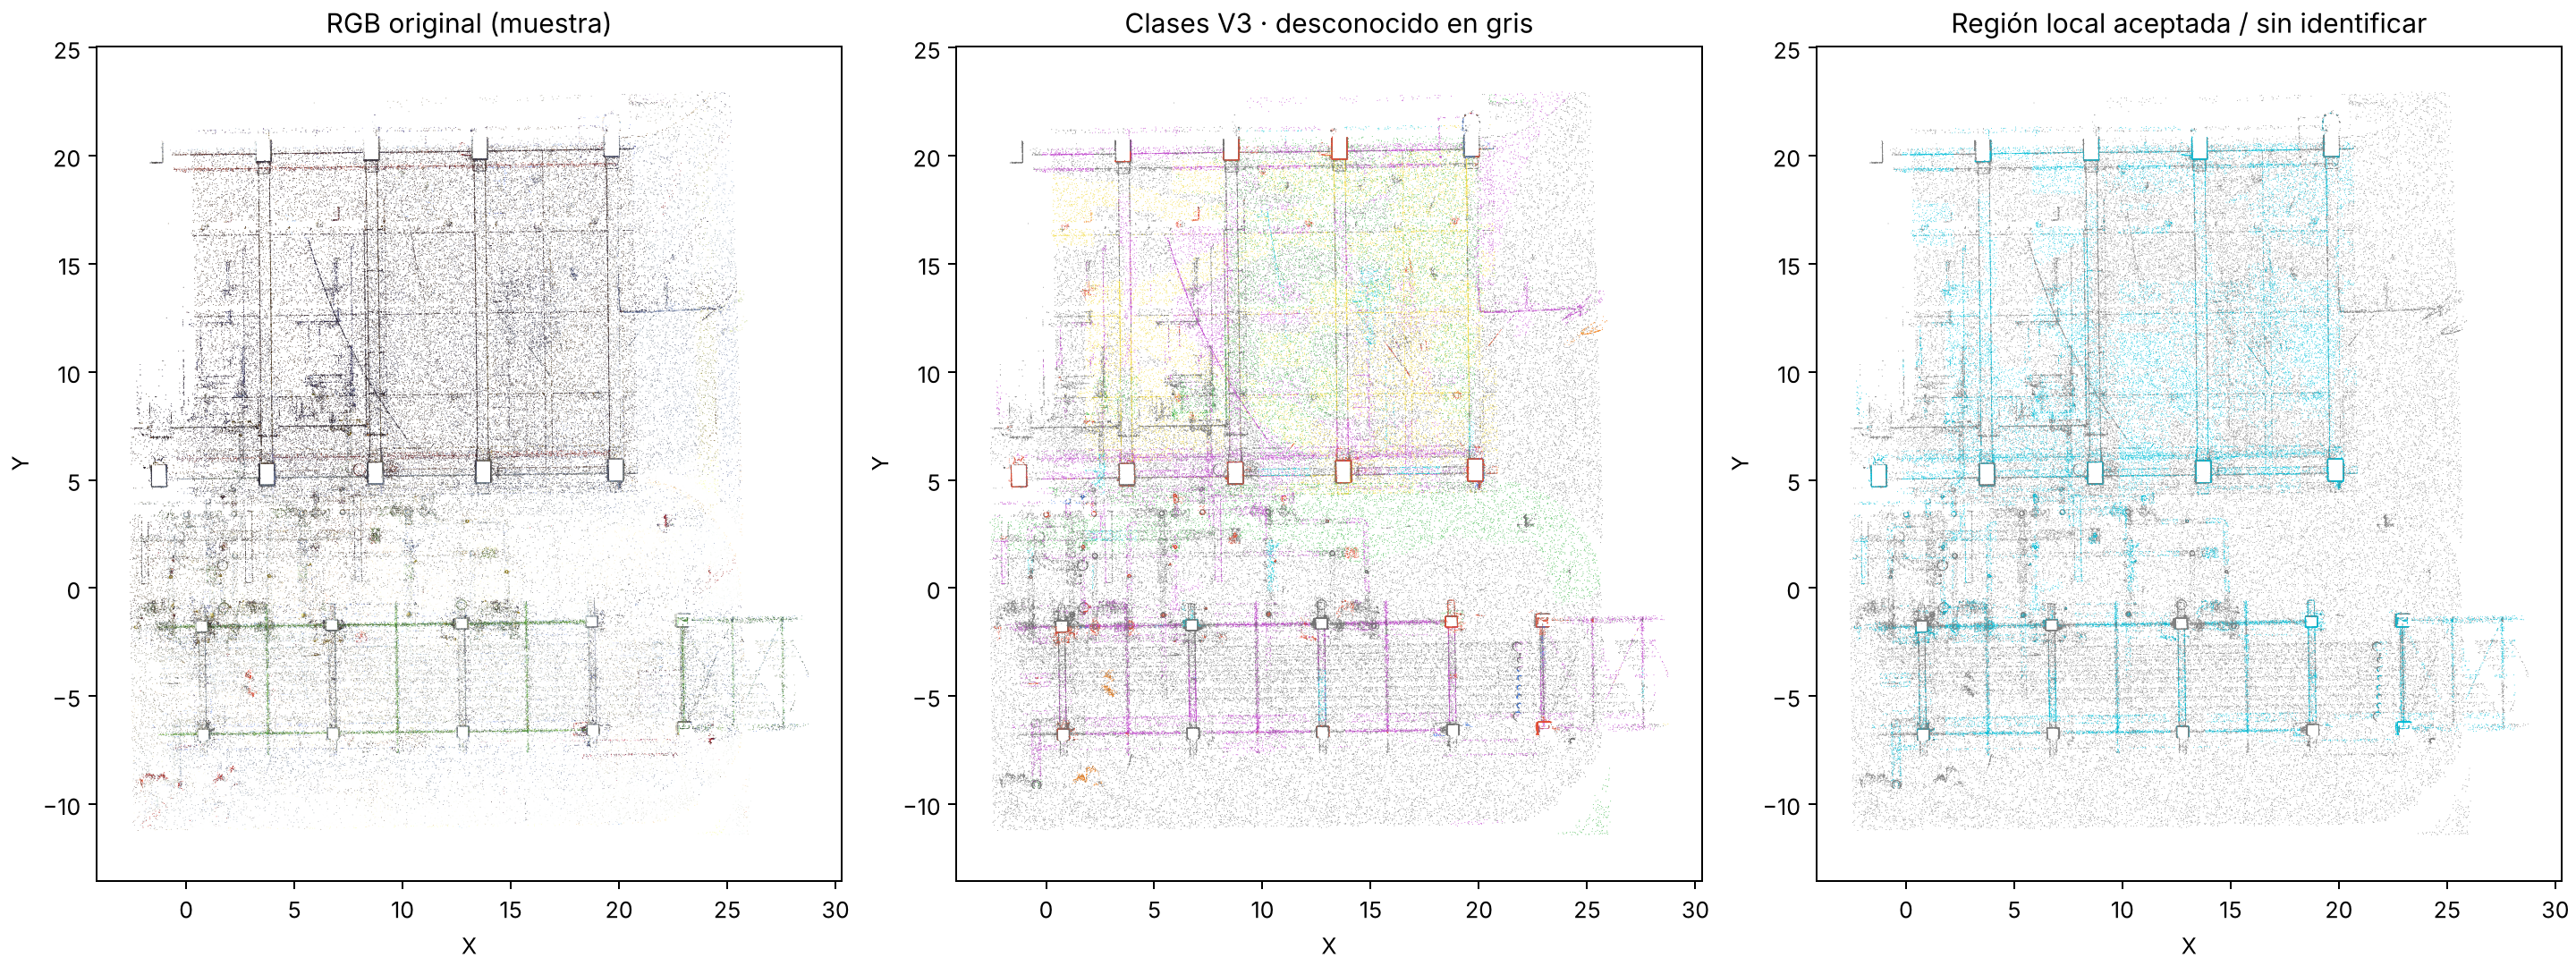
\includegraphics[width=\linewidth]{figures/fig6.png}
\caption{Comparación en planta: RGB original, clases V3 y regiones locales aceptadas por el refinamiento.}
\end{figure}
\begin{figure}[H]
\centering
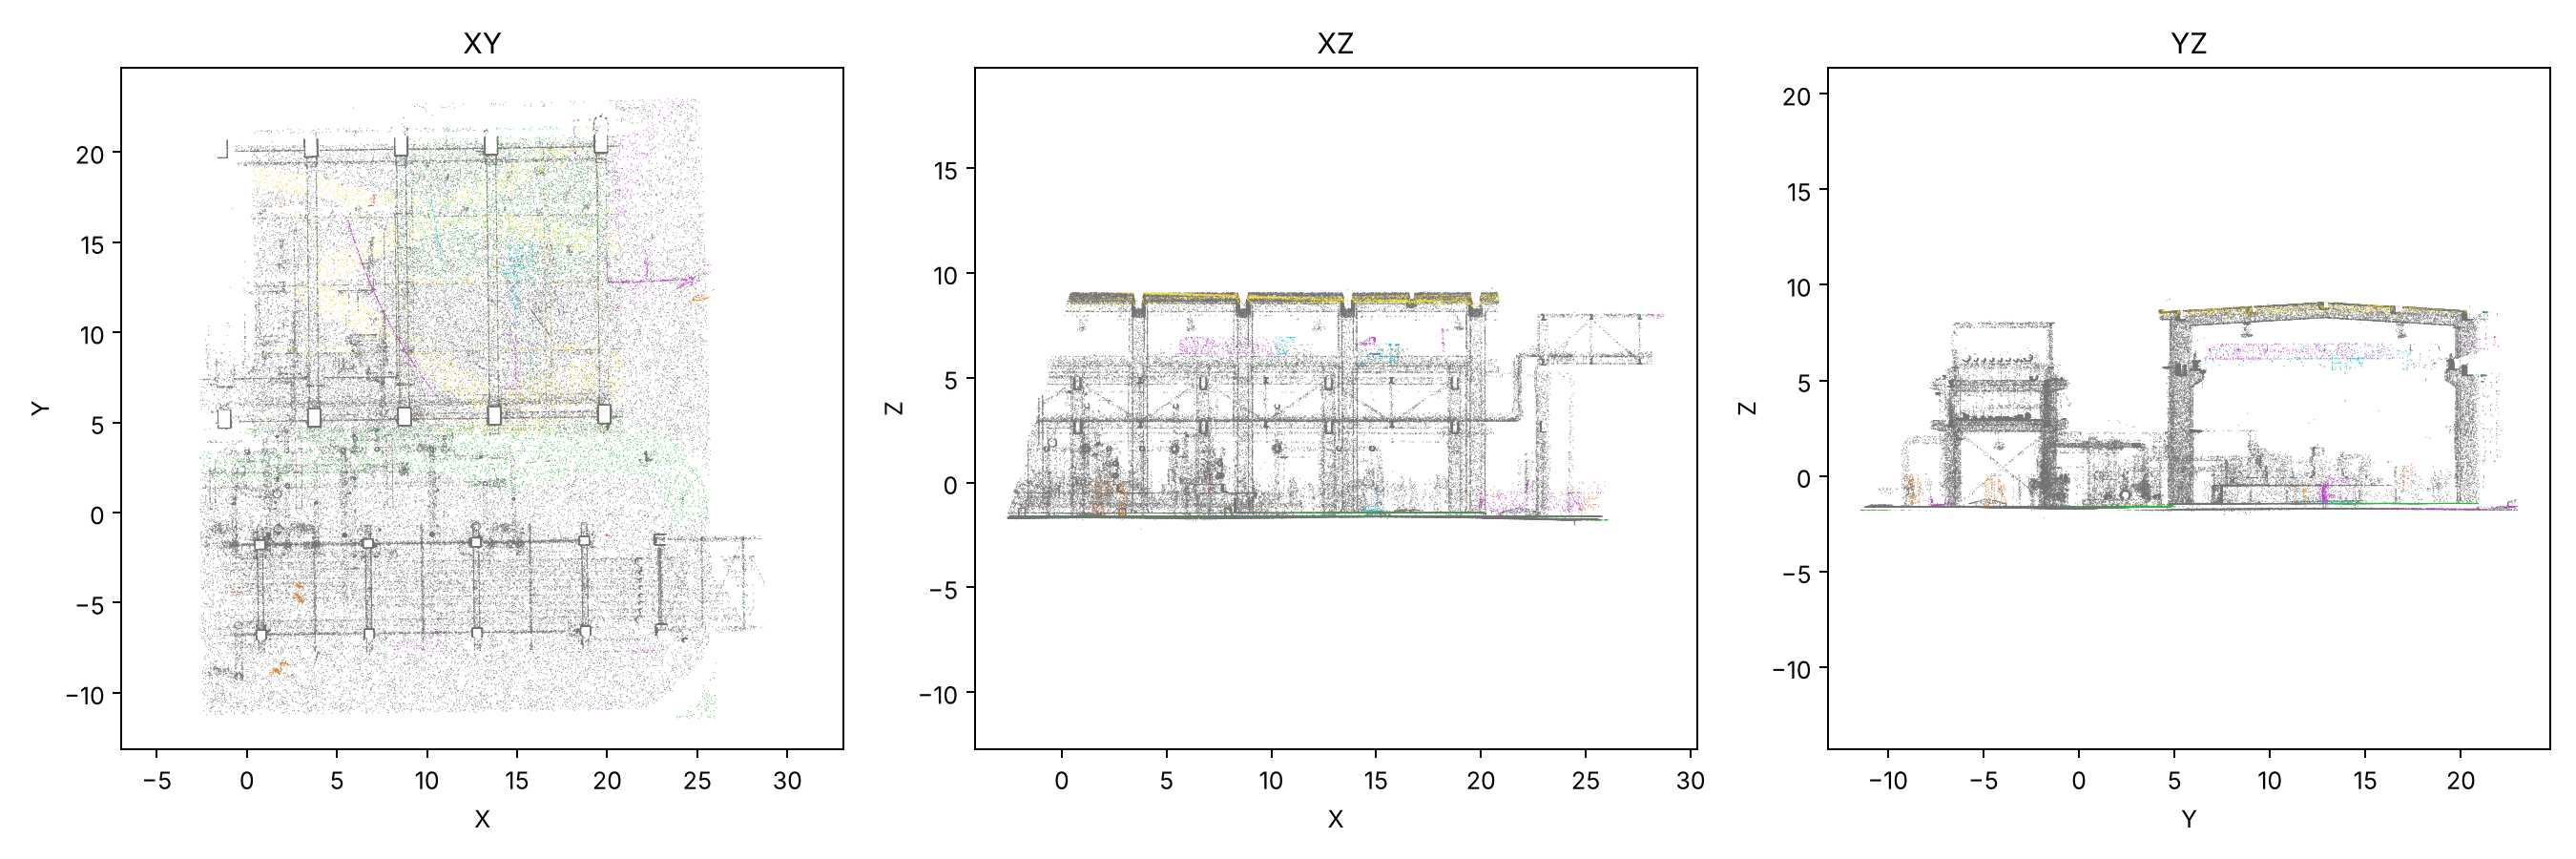
\includegraphics[width=\linewidth]{figures/fig7.png}
\caption{Proyecciones de la clasificación V1 (antes del refinamiento V3), para contraste.}
\end{figure}

\section{Limitaciones y trabajo futuro}
\begin{itemize}
\item \textbf{Cobertura baja:} el 57,2\,\% de los puntos queda sin clase. El componente gigante y los umbrales fijos limitan los resultados.
\item \textbf{Clases ausentes:} no se identifican personas ni vehículos; el vocabulario de clases del clasificador no los incluye.
\item \textbf{Sin verdad de referencia:} no hay anotaciones, por lo que la evaluación es cualitativa y de cobertura.
\item \textbf{Reglas manuales:} los umbrales (por ejemplo 0,22 y 0,78 de altura relativa) se fijaron a mano y dependen de la hipótesis de que $z$ es vertical.
\item \textbf{Comparación de algoritmos acotada:} se comparó k-means, GMM, Ward y DBSCAN sobre muestras de 10\,000 puntos con métricas internas (sección~\ref{sec:comparacion}); no se usaron en la segmentación entregada ni se evaluaron contra etiquetas reales.
\item \textbf{Mejoras posibles:} anotar a mano una muestra de puntos para calcular IoU y ARI; usar HDBSCAN o clustering sobre las variables de forma y color (sin posición) para separar el componente gigante; y ajustar los umbrales de las reglas con esa muestra anotada.
\end{itemize}
\paragraph{Reproducibilidad.} El pipeline completo se ejecutó con Python 3.12 y Open3D 0.20 y reprodujo las cifras de este reporte. La instalación con \texttt{uv sync} desde cero no se verificó en este entorno. La comparación de la sección~\ref{sec:comparacion} usa solo NumPy, scikit-learn y matplotlib, con semillas fijas.

\section{Conclusiones}
Se construyó un pipeline en varias etapas que combina voxelización, detección de planos con RANSAC, agrupamiento espacial por conectividad, descriptores de forma por PCA y clasificación por reglas, y que exporta una nube PLY con un color por clase. El resultado identifica de forma coherente los elementos estructurales dominantes (piso, techo, columnas y vigas), pero deja más de la mitad de los puntos sin clase y no distingue personas ni vehículos. Durante la integración se detectó y corrigió un error de escala en la altura relativa que impedía reconocer el techo. La comparación experimental mostró que los algoritmos de clustering clásicos, aplicados de forma global sobre las 13 variables, no separan clases bien definidas (silhouette máxima de 0,28) y que la posición domina el agrupamiento; esto respalda el diseño por etapas con reglas interpretables.

\section*{Referencias y atribución}
Open3D (lectura y escritura de PLY, RANSAC de planos); scikit-learn (DBSCAN como referencia y algoritmos de la sección~\ref{sec:comparacion}); formato PLY. El README del repositorio indica que el sistema de segmentación integra código del repositorio Jhynfe/Actividad\_3\_ML, con su historial conservado; el repositorio no incluye licencia. La nube de puntos pertenece a la actividad del curso y no se redistribuye en el repositorio.

\end{document}
